The target domain of the CORDET Framework are service-oriented applications. 
This section defines the service concept assumed in the CORDET Project (the \textit{CORDET Service Concept}).

A \textit{service} is a set of logically and functionally related capabilities that an application offers to other applications. 
The CORDET Service concept sees an application as a \textit{provider of services} to other applications and as a \textit{user of services} from other applications (see figure \ref{fig:ServConcept}).

A service is identified by its \textit{type}. 
The service type is a positive integer which uniquely identifies the service within the CORDET world and thus acts as a name for the service.

\begin{figure}[ht]
 \centering
 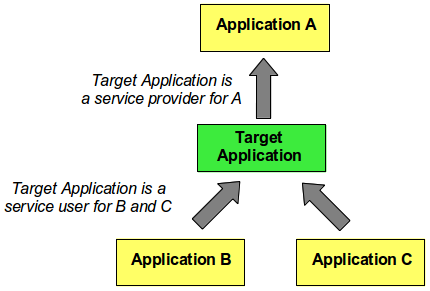
\includegraphics[scale=0.55,keepaspectratio=true]{ServConcept.png}
 \caption{Applications as Providers and Users of Services}
 \label{fig:ServConcept}
\end{figure}

The user of a service controls the service by sending \textit{commands} to the service provider. 
A command is a data exchange between a service user and a service provider to start, advance, modify, terminate, or otherwise control the execution of a particular activity within the service provider (see reference \cite{ref:pus}, section 3.1.13). 

The provider of a service sends \textit{reports} to the user of the service. 
A report is a data exchange between a service provider (the report initiator) and a service user to provide information relating to the execution of a service activity (see reference \cite{ref:pus}, section 3.1.14).

Thus, a service consists of a set of commands which the user of the service sends to the provider of the service and of a set of reports which the service provider sends back to its user. 
A command defines actions to be executed by the service provider. 
A report encapsulates information about the internal state of the service provider (see figure \ref{fig:ServCmdRep}).

\begin{figure}[ht]
 \centering
 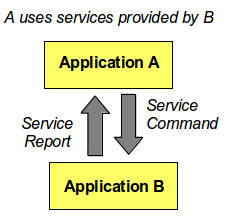
\includegraphics[scale=0.5,keepaspectratio=true]{ServCmdRep.png}
 \caption{Services as Sets of Commands and Reports}
 \label{fig:ServCmdRep}
\end{figure}

The same application may act as as a service provider to several user applications and, vice-versa, it may use the services from several other providers. For instance, in figure \ref{fig:ServConcept}, the Target Application has one user (Application A) and it acts as user for two service providers (Applications B and C). 

Figures \ref{fig:ServConcept} and \ref{fig:ServCmdRep} show situations where the service provider and service users have a direct connection but the CORDET Service Concept also supports situations where the connection between provider and user is indirect.

In figure \ref{fig:ServRerouting}, for instance, application A sends a command to application C but the command is routed through application B. 
Thus, the CORDET Service Concept can be used as a basis for the definition of distributed applications which interact with each other by exchanging service requests over a network. 

The network defines physical links between the applications in the system (e.g. the links between applications A and B and between applications B and C in figure \ref{fig:ServRerouting}) and the CORDET infrastructure defines logical links between the applications (e.g. the link between applications A and C).

\begin{figure}[ht]
 \centering
 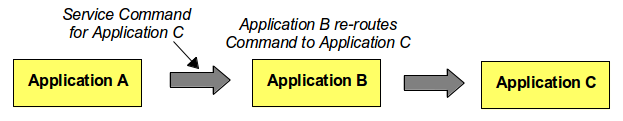
\includegraphics[scale=0.5,keepaspectratio=true]{ServRerouting.png}
 \caption{Re-Routing of Service Requests}
 \label{fig:ServRerouting}
\end{figure}

